\documentclass{article}


\PassOptionsToPackage{round}{natbib}
\usepackage[final]{neurips_2022}


\usepackage[utf8]{inputenc} % allow utf-8 input
\usepackage[T1]{fontenc}    % use 8-bit T1 fonts
\usepackage[colorlinks,citecolor=cyan,pagebackref=true,breaklinks=true,bookmarks=false]{hyperref}
\usepackage{url}            % simple URL typesetting
\usepackage{booktabs}       % professional-quality tables
\usepackage{amsfonts}       % blackboard math symbols
\usepackage{nicefrac}       % compact symbols for 1/2, etc.
\usepackage{microtype}      % microtypography
\usepackage{xcolor}         % colors



\title{Likelihood training of Schrödinger bridge using Forward-backward SDEs theory}


% The \author macro works with any number of authors. There are two commands
% used to separate the names and addresses of multiple authors: \And and \AND.
%
% Using \And between authors leaves it to LaTeX to determine where to break the
% lines. Using \AND forces a line break at that point. So, if LaTeX puts 3 of 4
% authors names on the first line, and the last on the second line, try using
% \AND instead of \And before the third author name.


\author{%
  Benjamin Maurel\\
  MVA - ENSAE\\
  École Normale Supérieure de Paris-Saclay\\
  Gif-sur-Yvettes, 91190, France\\
  \texttt{benjamin.maurel@ensae.fr}\\
  % examples of more authors
  \And
  Jérémie Stym-Popper\\MF
  MVA - ENSAE\\
  École Normale Supérieure de Paris-Saclay\\
  Gif-sur-Yvettes, 91190, France\\
  \texttt{jeremie.stym-popper@ensae.fr}\\
  \And
  Gabriel Watkinson\\
  MVA - ENSAE\\
  École Normale Supérieure de Paris-Saclay\\
  Gif-sur-Yvettes, 91190, France\\
  \texttt{gabriel.watkinson@ensae.fr}\\
}

% \usepackage[square,numbers]{natbib}         % Pour la bibliographie
\usepackage[nottoc]{tocbibind}
\usepackage{url}            % Pour citer les adresses web
\usepackage[hidelinks]{hyperref}       % Pour activer les liens cliquables
\usepackage[T1]{fontenc}    % Encodage des accents
\usepackage[utf8]{inputenc} % Lui aussi
\usepackage[english]{babel} % Pour la traduction française
\usepackage{numprint}       % Histoire que les chiffres soient bien
\usepackage{eurosym}        % Permet l'utilisation du signe € : \EUR{\num{299792458.38}}
\usepackage{appendix}       % Pour avoir des appendices
\usepackage{xspace}         % Utile lors de la création d'abréviations
\usepackage[dvipsnames]{xcolor}         % Permet de gérer facilement les couleurs.
\usepackage{verbatim}       % Permet d'insérer du code LaTeX sans qu'il soit compilé


% Setup du headers
\usepackage{fancyhdr}       % Fancy headers (page et titre de la section en haut)

\usepackage{etoolbox}


% Package pour avoir la section Annexes
\usepackage{appendix}
\renewcommand{\appendixtocname}{Appendix}  % On renomme dans la table des matières
\renewcommand{\appendixpagename}{Appendix} % On renomme dans le document

% Packages pour images et graphiques
\usepackage{graphicx}   % Inclusion des graphiques
\usepackage{graphics}
\usepackage{wrapfig}    % Dessins dans le texte.
\usepackage[justification=centering]{caption}    % Permet de personnaliser les styles des légendes.
\usepackage{subcaption} % Permet d’insérer au sein d’une figure des sous-figures, chacune d’entre elles disposant d’une légende, en plus de la légende principale.

% Un package pour les dessins (utilisé pour l'environnement {code})
\usepackage{tikz}
\usetikzlibrary{shapes.geometric, arrows}
\usepackage[framemethod=TikZ]{mdframed}

% Packages pour la création de nouvelles commandes
\usepackage{xifthen}
\usepackage{xargs}

% Packages pour la typographie
\usepackage[maxlevel=3]{csquotes} % Propose des commandes pour les citations. L'option maxlevel permet de déterminer le nombre de niveaux d'imbrication maximal.
% Exemple :  \enquote{Lorsque yyy déclare \enquote{zzz} il ne déclare rien du tout}. Les citations en bloc sont également possible : \begin{quote} citation \end{quote}. Pour les citations plus longues, on préférera \begin{quotation} citation longue \end{quotation}.
\usepackage{setspace}             % Permet de modifier l'espacement entre les lignes.


% Packages pour les mathématiques
\usepackage{amsmath}        % La base pour les maths
\usepackage{mathrsfs}       % Quelques symboles supplémentaires
\usepackage{amssymb}        % encore des symboles.
\usepackage{amsfonts}       % Des fontes, eg pour \mathbb.
\usepackage{mathtools}      % Permet d'utiliser des symboles d'égalités spéciaux
% \usepackage{dsfont}         % Pour avoir les notations nécessaires aux ensembles (nécessite mathbb)
% \usepackage{stmaryrd}       % Permet de faire des intervalles avec des doubles barres (intervalles d'entiers)
% \usepackage{esvect}         % Donne plein de possibilité pour les flèches des vecteurs
% \usepackage{systeme}        % Permet de créer facilement des systèmes (en mode mathématique ou en texte)

\usepackage{tcolorbox}
\usepackage{enumitem}
% \usepackage{witharrows}
%%%%%%%%%%%%%%%%%%%%%%%%%%%%%%%%%%%%%%%%%%%%%%%%
% Ce fichier contient des nouvelles commandes
% pour faciliter l'écriture des mathématiques
%%%%%%%%%%%%%%%%%%%%%%%%%%%%%%%%%%%%%%%%%%%%%%%%

% Ensembles
\let\ensembleNombre\mathbb
\newcommand*\N{\ensuremath{\ensembleNombre{N}}}       % Ensemble des entiers naturels N
\newcommand*\Z{\ensuremath{\ensembleNombre{Z}}}       % Ensemble des entiers relatifs Z
\newcommand*\Q{\ensuremath{\ensembleNombre{Q}}}       % Ensemble des rationnels Q
\newcommand*\R{\ensuremath{\ensembleNombre{R}}}       % Ensemble des réels R
\newcommand*\Complex{\ensuremath{\ensembleNombre{C}}} % Ensemble des complexes C

% Encadrement
\newcommand{\angles}[1]{\left\langle #1 \right\rangle} % ⟨⟩
\newcommand{\braces}[1]{\left\lbrace #1 \right\rbrace} % {}
\newcommand{\bracks}[1]{\left\lbrack #1 \right\rbrack} % []
\newcommand{\pars}[1]{\left( #1 \right)}               % ()
\newcommand{\norme}[2][]{\ensuremath{\left\Vert #2\right\Vert_{#1}}}       % Norme
\newcommand{\ent}[1]{\left\lfloor #1\right\rfloor}     % Partie entière inférieure
\newcommand{\entsup}[1]{\left\lceil #1\right\rceil}    % Partie entière supérieure
\newcommand{\abs}[1]{\left\vert #1\right\vert}         % Valeur absolue

% Dérivées
\newcommand{\deriv}[3][]{\frac{\mathrm{d}^{#1}#2}{\mathrm{d} {#3}^{#1}}}    % Dérivée non partielle
\newcommand{\partiald}[3][]{\frac{\partial^{#1}#2}{\partial {#3}^{#1}}} % Dérivée partielle

% Intervalles
\newcommand*\intervalle[4]{\left#1 #2 \, ; #3 \right#4}                       % Définit la notion d'intervalle
\newcommand*\intervalleOO[2]{\intervalle{]}{#1}{#2}{[}}                       % ]a ; b[
\newcommand*\intervalleFF[2]{\intervalle{[}{#1}{#2}{]}}                       % [a ; b]
\newcommand*\intervalleOF[2]{\intervalle{]}{#1}{#2}{]}}                       % ]a ; b]
\newcommand*\intervalleFO[2]{\intervalle{[}{#1}{#2}{[}}                       % [a ; b[
\newcommand*\intervalleEntier[2]{\intervalle{\llbracket}{#1}{#2}{\rrbracket}} % Ensemble d'entiers

% Ensemble "tel que"
\newcommand*\enstq[2]{\braces{#1\;|\; #2}}

% Probabilité, espérance, variance, covariance et corrélation
\newcommandx{\proba}[3][1, 3=0]{
\ifthenelse{\isempty{#2}}{\mathbb{P}_{#1}}{%
\ifthenelse{\equal{#3}{0}}{\mathbb{P}_{#1}\pars{#2}}{\mathbb{P}_{#1}\pars{#2 \middle| #3}}}%
}
\newcommandx{\esp}[3][1, 3=0]{
\ifthenelse{\isempty{#2}}{\mathbb{E}_{#1}}{%
\ifthenelse{\equal{#3}{0}}{\mathbb{E}_{#1}\bracks{#2}}{\mathbb{E}_{#1}\bracks{#2 \middle| #3}}}%
}
\newcommandx{\var}[3][1, 3=0]{
\ifthenelse{\isempty{#2}}{\operatorname{Var}_{#1}}{%
\ifthenelse{\equal{#3}{0}}{\operatorname{Var}_{#1}\pars{#2}}{\operatorname{Var}_{#1}\pars{#2 \middle| #3}}}%
}
\newcommandx{\cov}[4][1, 4=0]{
\ifthenelse{\isempty{#2} \AND \isempty{#3}}{\operatorname{Cov}_{#1}}{%
\ifthenelse{\equal{#4}{0}}{\operatorname{Cov}_{#1}\pars{#2, #3}}{\operatorname{Cov}_{#1}\pars{#2, #3 \middle| #4}}}%
}
\newcommandx{\corr}[3][1]{\ifthenelse{\isempty{#2} \AND \isempty{#3}}{\operatorname{Corr}_{#1}}{\operatorname{Corr}_{#1}\pars{#2, #3}}}

% Lois usuelles de probabilités
\newcommand{\Ber}[1]{\mathcal{B}ernoulli\pars{#1}}       % Bernoulli
\newcommand{\Binom}[2]{\mathcal{B}\pars{#1, #2}}         % Binomiale
\newcommand{\Poisson}[1]{\mathcal{P}\pars{#1}}           % Poisson
\newcommand{\Geo}[1]{\mathcal{G}eo\pars{#1}}             % Géométrique
\newcommand{\Unif}[1]{\mathcal{U}nif_{#1}}               % Uniforme
\newcommand{\Exp}[1]{\mathcal{E}xp\pars{#1}}             % Exponentielle
\newcommandx{\Norm}[3][1]{\mathcal{N}_{#1}\pars{#2, #3}} % Normale
\newcommand{\Gammaloi}[2]{\Gamma\pars{#1, #2}}           % Gamma
\newcommand{\Betaloi}[2]{\beta\pars{#1, #2}}             % Beta
\newcommand{\Pareto}[2]{\mathcal{P}areto\pars{#1, #2}}   % Pareto
\newcommand{\Laplace}[1]{\mathcal{L}\pars{#1}}           % Laplace
\newcommand{\Cauchy}[1]{\mathcal{C}\pars{#1}}            % Cauchy

% Égalités
\newcommandx{\egalloi}{\overset{\mathrm{\mathcal{L}oi}}{=}} % égalité en loi
\newcommandx{\egalprob}{\overset{\mathbb{P}}{=}}            % égalité en probabilité
\newcommandx{\egaltxt}[1]{\overset{\mathrm{#1}}{=}}         % égal avec overscript
\newcommandx{\simiid}{\overset{\mathrm{iid}}{\sim}}         % sim iid

% Indicatrice
\newcommand{\1}[1][]{\mathds{1}_{#1}}

% max, min, argmax et argmin avec subscript
\newcommandx{\maxx}[1]{\underset{#1}{\max}}
\newcommandx{\minn}[1]{\underset{#1}{\min}}
\newcommandx{\argmax}[1][1]{\underset{#1}{\arg\max}}
\newcommandx{\argmin}[1][1]{\underset{#1}{\arg\min}}

% matrice 3*3 diagonale avec la diagonale donnée sur les 3 arguments
\newcommand{\mattroisdiag}[3]{\left( \begin{array}{ccc} #1 &  0 &  0 \\ 0  & #2 &  0 \\ 0  &  0 & #3\end{array} \right)}

% Intégration
\newcommand{\dint}{\mathrm{d}}
\newcommandx{\integ}[4][2]{\int_{#1}^{#2} #3 \, \mathrm{d} #4}

% moyenne simple et quadratique d'une grandeur scalaire
\newcommand{\moy}[1]{\overline{#1}}
\newcommand{\moyy}[1]{\overline{#1^2}}

% Vecteurs
\let\vecteur\overrightarrow % Permet de modifier la taille de la flèche d'un vecteur quand ce dernier est composé de plusieurs lettres par exemple.
\newcommand*\coord[2]
{
   \vecteur{#1} \,
   \begin{pmatrix}
      #2
   \end{pmatrix}
} % Permet de déclarer les coordonnées d'un vecteur, exemple : \[\coord{AB}{12\\21} \coord{BC}{21\\12\\32}\]

% Surface et volume
\newcommandx{\surf}[2][2=m]{\numprint{#1}\,#2\textsuperscript{2}}
\newcommandx{\vol}[2][2=m]{\numprint{#1}\,#2\textsuperscript{3}}

% Fonction
\newcommand*\fonction[5]{
#1 \colon \left\{\begin{alignedat}{2}  &#2 &\: &\to      #3\\
                                &#4 &   &\mapsto  #5
\end{alignedat} \right. \kern-\nulldelimiterspace} % Permet de déclarer facilement une fonction, exemple : $\fonction{f}{E}{F}{x}{f(x)}$

% Autres commandes utiles
\newcommand{\compos}{\circ}                 % operateur de composition de fonctions
\DeclareMathOperator{\card}{card}           % On déclare l’opérateur \card qui correspond à « card ».
\newcommand*\PI{\ensuremath{\pi}}           % Permet d'afficher pi que l'on soit en mode math ou non.
\newcommand{\ds}[1]{\displaystyle{#1}}      % Force LaTeX à gérer les indices et les exposants comme si il était en mode mathématique isolé
\newcommand{\kronecker}[0]{\mathrm{\delta}} % symbole de Kronecker
\newcommand{\heaviside}[0]{\mathrm{H}}      % fonctions d'Heaviside
\newcommand{\dirac}[0]{\mathrm{\delta}}     % Distribution de Dirac
\newcommand{\Zt}{\ensuremath{\textbf{Z}_t}\xspace}

\begin{document}

\maketitle


\section*{Introduction}

\let\thefootnote\relax\footnote{Link to our GitHub: \url{https://github.com/gwatkinson/mva_sb_generative}, containing code of our experiments and further images and resources}

Scored-based Generative Models (SGMs) have gained significant attention in the field of deep image generation.
Since their introduction by \citet{song2020score}, SGMs have emerged as the state-of-the-art approach for image generation.
Unlike likelihood-based models such as VAEs or normalizing flows, which learn the probability density function directly, or adversarial-based models like GANs,
SGMs learn a mapping between a simple distribution, typically Gaussian, and a complex, high-dimensional, and often intractable data distribution, such as images.
These models offer several advantages over existing approaches, including high-quality sample generation comparable to GANs without the instability of adversarial training, flexible model architectures and the ability to solve inverse problems without re-training models.
However, SGMs also suffer from pitfalls that limit their applicability, such as difficult training procedure, the impossibility to use a complex distribution as the prior, the fact that the drift can only be linear or degenerate, and slow training and sampling processes compared to other methods.

To address these limitations, recent works by \cite{debortoli2023diffusion, pmlr-v139-wang21l, vargas2021solving} have proposed a new class of generative models inspired by Optimal Transport theory, specifically using Schrödinger Bridges (SB) \cite{schrodinger1932theorie}.
SBs, similar to SGMs, aim to learn a mapping between two distributions in a finite horizon.
However, SBs offer greater flexibility by allowing the mapping between arbitrary distributions, making them more appealing.
The relationship between SBs and SGMs was not clearly established, as SGMs rely on Stochastic Differential Equations (SDEs), whereas SBs are based on Partial Differential Equations (PDEs).

In this paper, \cite{chen2023likelihood} bridges the gap between these seemingly distinct mathematical concepts by drawing inspiration from the field of Stochastic Optimal Control and utilizing Forward-Backward Stochastic Differential Equations (FBSDEs).
The authors propose a method that enables the solution of PDEs with SDEs, offering computational efficiency and improved precision compared to solving PDEs directly.
This approach introduces a novel training method for SBs, resembling the framework used in flow-based diffusion models.
Additionally, the authors also use a more traditional Iterative Proportional Fitting approach (IPF; \cite{kullback1968probability,debortoli2023diffusion}).

In this report, we will first introduce the two classical methods, Scored-based Generative Models and Schrödinger Bridges, before exploring the Forward-Backward Stochastic Differential Equations method that establishes a connection between the two.
Finally, we will discuss further extensions of this paper, including an application of the method with the Hamilton-Jacobi-Bellman PDE.



\section{Some reminders about Score-based Generative Model}

Given a dataset $\braces{\mathbf{x}_1, \mathbf{x}_2, \dots, \mathbf{x}_N}$ of $N$ samples in $\mathbb{R}^d$, the goal of generative models is to learn the underlying data distribution $p_\mathrm{data}$, as to be able to generate new samples from this distribution.
The go-to approach for this kind of problem is to use maximum likelihood estimation (MLE) to learn the parameters of a parametric model $p_\theta$ that approximates the distribution. However, this relies on the assumption that $p_\theta$ be a normalized density function. To do so, we have to calculate the normalizing constant, which is intractable in high dimension. Therefore, to train such models using MLE, we either have to restrict the architectures, e.g. to invertible networks in flow models, or approximate the normalizing constant, using MCMC methods for example. This is not ideal, as it limits the flexibility of the model and the quality of the approximation.

Another solution is to use the score function $s_\theta(x) = \nabla_x \log p_\theta(x)$ instead of the density function $p_\theta$.
This makes the normalization constant disappear thanks to the gradient, allowing a wider range of architectures.
Score matching methods can then be used to learn the score function $s_\theta$, followed Langevin dynamics to sample from the learned score function, giving access to the wanted distribution.
However, this naive approach doesn't work well in practice, especially in low density regions.

The solution is to add a diffusion process to the score matching method, which is the idea behind Score-based Generative Models (SGM).
In SGMs, inputs are "diffused" toward a random noise.
This diffusion process is characterized by a stochastic differential equation (SDE):
\begin{equation}
    \dint{\mathbf{X}_t} = f(t,\mathbf{X}_t)\dint{t} + g(t) \dint{\mathbf{W}_t}, \quad \mathbf{X}_0 \sim p_\mathrm{data}
    \label{eq:forward_sde_sgm}
\end{equation}
where $f(\cdot, t) : \R^n \rightarrow \R^n$, $g(t) \in \R$ are the drift and diffusion coefficients, and $\mathbf{W}_t \in \R^n$ is a standard Wiener process.
For a large time step, we have that $p_T \approx p_\mathrm{prior}$ that closely resemble a Gaussian distribution, which is easy to sample from.

The associated backward SDE is:
\begin{equation}
    \dint{\mathbf{X}_t} = \bracks{f(t,\mathbf{X}_t) - g(t)^2\nabla_x\log p_t(\mathbf{X}_t)}\dint{t} + g(t) \dint{\mathbf{W}_t}, \quad \mathbf{X}_T \sim p_T
    \label{eq:backward_sde_sgm}
\end{equation}

The score function appears naturally in the backward SDE, which is the reason why SGMs are called score-based. In the case where the drift is simple (e.g. linear or degenerate), it is possible to learn a score network $s(t, x; \theta)$ by regressing the outputs to the ground truth, i.e $\esp{\lambda(t) \norme{s(t, x; \theta) - \nabla_x \log p_{t|x_0}}^2}$, where the expectation is taken over the forward SDE.
$\lambda(t)$ is a weighting function that is crucial in practice, but hard to choose well.

More recently, \citet{song2021maximum} have found a lower-bounds to the log-likelihood of the SGM, resulting in an Evidence Lower bound (ELBO) :
\begin{equation}
\label{eq:sgm_logl}
\log p_0^\mathrm{SGM}(\mathbf{x}_0)
\ge
\esp{\log p_T(\mathbf{X}_t)}
- \int_0^T
\esp{\frac{1}{2}g^2\norme{\mathbf{s}_t}^2
- \nabla_x \cdot (g^2 s_t - f)}
\dint t
\end{equation}
This can be obtained bounding the KL divergence by score-matching loss, where the weighting function $\lambda(t) = g(t)^2$.
This lower bound is important since it will be one of the element that links together the SGM model and the Schrödinger-Bridge problem.

Once the model is trained, we can just substitute the score function by the learned one in the backward SDE \eqref{eq:backward_sde_sgm} to sample from the data distribution.




\section{Schrödinger Bridge}

Unlike SGMs, Schrödinger Bridges (SB) are not generative models, but rather a way to interpolate between two distributions $\mu_0$ and $\mu_1$.
There were first introduced by \citet{schrodinger1932theorie} and are related to the field of regularized optimal transport.
The Schrödinger Bridge problem can be defined as follows:
\begin{equation*}
    \Pi^\star = \argmin\braces{\mathrm{KL}(\Pi|\mathbb{P}) \, | \, \Pi \in \mathcal{P}(\mathcal{C}), \, \Pi_0 = p_{\textrm{data}}, \, \Pi_T = p_{\textrm{prior}}}
\end{equation*}
where $\Pi^0$ is the reference measure, which is set to the path measure of the forward diffusion process in \eqref{eq:forward_sde_sgm}.

The \textbf{Benamou-Brenier} reformulation of the entropy-regularized optimal transport problem gives the following partial differential equations (PDEs):
\begin{equation}
    \label{eq:sb_pdes}
    \begin{cases}
    \frac{\partial \Psi}{\partial t} = -\nabla_x \Psi^\top f - \frac{1}{2}\mathrm{Tr}(g^2 \nabla_x^2 \Psi) \\[7pt]
    \frac{\partial \widehat{\Psi}}{\partial t} = -\nabla_x \cdot (\widehat{\Psi} f) + \frac{1}{2}\mathrm{Tr}(g^2 \nabla_x^2 \widehat{\Psi})
    \end{cases}
    \mathrm{s.t.}
    \begin{array}{lcl}
        \Psi(0, \cdot) \widehat{\Psi}(0, \cdot) &=& p_\mathrm{data}\\
        \Psi(T, \cdot) \widehat{\Psi}(T, \cdot) &=& p_\mathrm{prior}
    \end{array}
\end{equation}
where $\Psi$ and $\widehat\Psi$ can also be seen as solutions to the Schrödinger system of equations (we recall that the trace of the Hessian is the Laplace operator). $f$ and $g$ are functions defined on the same space as above.

If $\Psi$ and $\widehat\Psi$ are solutions of these PDEs, then the solution of the SB problem is the path measure (i.e, that is in $\mathcal{P}(p_\mathrm{data}, p_\mathrm{prior})$ of the following SDEs:
\begin{equation}
    \label{eq:sb_sdes}
\begin{aligned}
    \dint\mathbf{X}_t & = \bracks{f+g^2\nabla_x\log\Psi(t,\mathbf{X}_t)}\dint t + g\dint \mathbf{W}_t, \quad \mathbf{X}_0 \sim p_\mathrm{data}\\
    \dint \mathbf{X}_t & = \bracks{f-g^2\nabla_x\log\widehat\Psi(t,\mathbf{X}_t)}\dint t + g \dint \mathbf{W}_t, \quad \mathbf{X}_T \sim p_\mathrm{prior}
\end{aligned}
\end{equation}
This establishes a first link between PDEs founding the SB problem and SDEs characterizing the SGM model.
Those SDEs are really similar to the ones of the SGM model, except for the terms $\nabla_x\log\Psi(t,\mathbf{X}_t)$ which adds non-linearity to the drift and $\nabla_x\log\widehat\Psi(t,\mathbf{X}_t)$ which can be seen as a modified score function.
In this situation, we have to learn both the score function and the drift function, while SGM only learns the score.

% The whole idea is to get rid of this term "$\nabla_x\log\widehat\Psi(t,\mathbf{X}_t)$" by adapting the ELBO loss.
To create samples using this method, we have to solve the PDEs \eqref{eq:sb_pdes} to obtain $\widehat\Psi$.
However, those are hard to solve, the proposed method of FBSDEs (Forward-Backward SDEs) is shown to be a convenient way to link the optimality conditions of the SB problem to the ELBO maximization of the likelihood $\log_0^\mathrm{SGM}(\mathbf{x}_0)$.




\section{Proposed Method}

There are two main methods to solve PDEs: linearization-based method and sampling-based method. The latter is a consequence of the Feynman-Kac lemma that provides a solution to parabolic PDEs with a conditional expectation (suitable for sampling), which establishes a link between this kind of PDE with stochastic processes. Here, the Nonlinear Feynman-Kac formula enables to link parabolic PDEs to forward-backward coupled SDEs as below. First, let's introduce a more general framework, so that \eqref{eq:forward_sde_sgm}, \eqref{eq:backward_sde_sgm} and \eqref{eq:sb_sdes} fall inside:
\begin{equation}
    \label{eq:general_sdes}
    % \label{eq:fbsde1}
    \begin{cases}
    \dint\mathbf{X}_t  = f(t,\mathbf{X}_t)\dint t + G(t,\mathbf{X}_t)\dint\mathbf{W}_t
    & \mathbf{X}_0 =\mathbf{x}_0 \\[5pt]
    \dint\mathbf{Y}_t = - h(t,\mathbf{X}_t, \mathbf{Y}_t,\mathbf{Z}_t)\dint t + \mathbf{Z}(t,\mathbf{X}_t)^\top \dint\mathbf{W}_t
    & \mathbf{Y}_T = \phi(\mathbf{X}_T)
    \end{cases}
\end{equation}

% \begin{equation}\label{eq:fbsde1}
% \left\{\begin{array}{ll}
%    \dint\mathbf{X}_t  & = f(t,\mathbf{X}_t)\dint t + G(t,\mathbf{X}_t)\dint\mathbf{W}_t, \quad \mathbf{X}_0 =\mathbf{x}_0  \\
%    \dint\mathbf{Y}_t & = - h(t,\mathbf{X}_t, \mathbf{Y}_t,\mathbf{Z}_t)\dint t + \mathbf{Z}(t,\mathbf{X}_t)^\top \dint\mathbf{W}_t,\quad \mathbf{Y}_T = \phi(\mathbf{X}_T).
% \end{array}\right.
% \end{equation}

Then, with the Itô Formula \citep{EXARCHOS2018159}, it is shown that if $\mathbf{v} \equiv v(t,\mathbf{X}_t)$ and $G(t,\mathbf{X}_t)$ are solution of the following PDE:
\begin{equation}
\label{eq:general_pde}
\frac{\partial v}{\partial t}
+ \frac{1}{2}\mathrm{Tr}(\nabla_\mathbf{x}^2 vGG^\top)
+ \nabla_\mathbf{x}v^\top f
+ h(t,\mathbf{x},v,G^\top\nabla_\mathbf{x}v)
= 0, \quad v(T,\mathbf{x}) = \phi(\mathbf{x})
\end{equation}

Then, with $\mathbf{Y}_t$ and $\mathbf{Z}_t$ the variables from \eqref{eq:general_sdes}, we have that :
\[
v(t,\mathbf{X}_t) = \mathbf{Y}_t \quad \text{and} \quad G(t,\mathbf{X}_t)^\top \nabla_\mathbf{x}v(t,\mathbf{X}_t) = \mathbf{Z}_t
\]

This give the possibility to solve either one of the problems, the SDEs \eqref{eq:general_sdes} or the second-order parabolic PDE \eqref{eq:general_pde}.
This is convenient computational wise, as the Forward-Backward SDE method \citep{pmlr-v120-pereira20a} provides a way to solve second-order parabolic PDE.

Similarly, instead of directly solving the PDEs linked to the SB problem, it is possible to solve the underlying forward and backward SDEs. Using this framework for SBs, we obtain that:
\begin{equation}
    \label{eq:sb_fbsde}
    \begin{cases}
        \displaystyle \dint\mathbf{X}_t = (f+g\mathbf{Z}_t) \dint t + g \dint \mathbf{W}_t
        \\[7pt]
        \displaystyle \dint\mathbf{Y}_t = \frac{1}{2}\mathbf{Z}_t^\top\mathbf{Z}_t\dint t + \mathbf{Z}_t^\top\dint\mathbf{W}_t
        \\[7pt]
        \displaystyle \dint\widehat{\mathbf{Y}}_t = \pars{
        \frac{1}{2}\widehat{\mathbf{Z}}_t^\top\widehat{\mathbf{Z}}_t
        + \nabla_\mathbf{x} . (g\widehat{\mathbf{Z}}_t - f)
        + \widehat{\mathbf{Z}}_t^\top \mathbf{Z}_t} \dint t
        + \widehat{\mathbf{Z}}_t^\top\dint\mathbf{W}_t
    \end{cases}
\end{equation}
where, in the second-order parabolic PDE \eqref{eq:general_pde}, $v$ is replaced with $\log \Psi$ and $\log\widehat\Psi$. The constraints are $X_0 = x_0$ and $\mathbf{Y}_T + \widehat{\mathbf{Y}}_T = \log p_{\rm prior}(\mathbf{X}_T)$.

Then, the nonlinear Feynman-Kac relations between the FBSDEs \eqref{eq:sb_fbsde} and PDEs \eqref{eq:sb_pdes} are:
\begin{equation*}
\begin{aligned}
    \mathbf{Y}_t = \log\Psi(t,\mathbf{X}_t), \quad \mathbf{Z}_t = g \nabla_\mathbf{x}\log \Psi(t,\mathbf{X}_t)\\
    \widehat{\mathbf{Y}}_t = \log\widehat\Psi(t,\mathbf{X}_t), \quad \widehat{\mathbf{Z}}_t = g\nabla_\mathbf{x}\log\widehat\Psi(t,\mathbf{X}_t)
\end{aligned}
\end{equation*}

We also get that $\mathbf{Y}_t + \widehat{\mathbf{Y}}_t = \log(\Psi(t,\mathbf{X}_t)\widehat\Psi(t,\mathbf{X}_t)) = \log p_t^\mathrm{SB}(\mathbf{X}_t)$.

Furthermore, by considering approximations of $\mathbf{Z}_t$ and $\widehat{\mathbf{Z}}_t$, with $g$ known (by design), it becomes possible to approximate $\nabla_x\log\widehat\Psi(t,\mathbf{X}_t)$ and $\nabla_x\log\Psi(t,\mathbf{X}_t)$. In this context, $\mathbf{Z}_t$ and $\widehat{\mathbf{Z}}t$ can be interpreted as policies that are learned to align the distributions $p_T$ and $p_\mathrm{prior}$. While this requirement is imposed in the SB model, it is not present in SGM, where the prior distribution is approximated. Consequently, $\mathbf{Z}_t$ directs the forward process towards the prior distribution, while $\widehat{\mathbf{Z}}_t$ adjusts the backward process accordingly.

From there, \cite{chen2023likelihood} show that, given a path sampled from the forward
SDE of \eqref{eq:sb_fbsde}, the solutions to the backward SDEs at $t = 0$ provide an unbiased estimation of the log-likelihood of the data point $x_0$:
\begin{equation}\label{9}\tag{9}
    \esp{\mathbf{Y}_0 + \widehat{\mathbf{Y}}_0|\mathbf{X}_0 = x_0} =
    \log p_0^\mathrm{SB}(x_0) =
    \log p_{\rm data}(x_0)
\end{equation}

Now, similarly to the log-likelihood of SGM models \eqref{eq:sgm_logl}, we have that:
\begin{align}
    \log p_0^\mathrm{SB}(x_0)
    &= \esp{\mathbf{Y}_T + \widehat{\mathbf{Y}}_T - \int_0^T \dint \mathbf{Y}_t + \mathbf{\widehat{Y}}_t\bigg\rvert\mathbf{X}_0 = x_0} \notag \\
    &= \esp{\mathbf{Y}_T + \widehat{\mathbf{Y}}_T|\mathbf{X}_0 = x_0}  \\
    & \quad \quad \quad - \int_0^T \esp{
    \frac{1}{2}\mathbf{Z}_t^\top\mathbf{Z}_t
    + \frac{1}{2}\widehat{\mathbf{Z}}_t^\top\widehat{\mathbf{Z}}_t
    + \nabla_\mathbf{x} . (g\widehat{\mathbf{Z}}_t - f)
    + \widehat{\mathbf{Z}}_t^\top \mathbf{Z}_t
    }
    \dint t \notag
    % \\
    % &= \esp{\log p_Y^\mathrm{SB}(\mathbf{X}_T)}
    % - \int_0^T \esp{
    % \frac{1}{2}  \norme{\mathbf{Z}_t}^2
    % + \norme{\widehat{\mathbf{Z}}_t}^2
    % + \nabla_x \cdot (g\widehat{\mathbf{Z}}_t - f)
    % + \widehat{\mathbf{Z}}_t^\top \mathbf{Z}_t}
    % \dint t
\end{align}


% \begin{align*}
% \esp{\mathbf{Y}_0 + \widehat{\mathbf{Y}}_0|\mathbf{X}_0 = x} & =  \nabla_x\log\widehat\Psi(t,\mathbf{x})\\
% \esp{\mathbf{Y}_0|\mathbf{X}_0 = x} &= \esp{\mathbf{Y}_T - \int_0^T \dint \mathbf{Y}_t \bigg\rvert\mathbf{X}_0 = x}\\
% \esp{\mathbf{Y}_0|\mathbf{X}_0 = x} & = \esp{\mathbf{Y}_T|\mathbf{X}_0 = x} -\int_0^T \pars{\esp{\int_0^T \frac{1}{2}\|\mathbf{Z}_t\|²\bigg\rvert\mathbf{X}_0 = x} + \esp{\mathbf{Z}_t \dint \mathbf{W}_t|\mathbf{X}_0 = x}}\dint t \\
% \esp{\widehat{\mathbf{Y}}_0|\mathbf{X}_0 = x} & = \esp{\widehat{\mathbf{Y}}_T|\mathbf{X}_0 = x} - \int_0^T \esp{\frac{1}{2}\|\widehat{\mathbf{Z}}_t\|^2 + \nabla_x \cdot (g\widehat{\mathbf{Z}}_t - f) + \widehat{\mathbf{Z}}_t^\top \mathbf{Z}_t}\dint t
% \end{align*}


This allows them to derive the theorem that solves all our issues:
\begin{equation}
\label{eq:logpSB}
\begin{aligned}
\log p_0^\mathrm{SB}(x_0) & = \esp{\log p_T(\mathbf{X}_T)}- \int_0^T \esp{\frac{1}{2}\|\mathbf{Z}_t\|^2 + \frac{1}{2}\|\widehat{\mathbf{Z}}_t\|^2 + \nabla_x \cdot (g\widehat{\mathbf{Z}}_t - f) + \widehat{\mathbf{Z}}_t^\top \mathbf{Z}_t} \dint t
\end{aligned}
\end{equation}

We now have an ELBO to maximize with every term tractable.
That allows us to use two trainable networks to learn the optimal controls $\mathbf{Z}_t^\theta$ and $\widehat{\mathbf{Z}}_t^\phi$ only, that are the optimal forward and backward drifts for SB.

This is a generalisation of SGM, indeed, for $(\mathbf{Z}_t^\theta, \widehat{\mathbf{Z}}_t^\phi) = (0, g s_t)$, the SB log-likelihood objective is the same as \eqref{eq:sgm_logl}. SBs allow for a wider array of drifts.



\section{Going further : SB FB-SDE to solve PDEs}

Neural networks can be trained to sample paths that solve partial differential equations (PDEs). In this section, we aim to explore the connection between the SB-FBSDE method and the solution of complex PDEs.



\subsection{An introduction to the Hamilton-Jacobi-Bellman PDE}

One widely known example of a PDE is the Hamilton-Jacobi-Bellman (HJB) equation. It is commonly used in optimal control theory, as its solution provides the sought-after value function for an optimal control problem. The HJB equation also plays a crucial role in dynamic programming by offering efficient methods for solving variational problems. The HJB PDE can be expressed as follows:


\begin{equation}
\frac{\partial V(t,x)}{\partial t} + \min_u\braces{\frac{\partial V(t,x)}{\partial x}\times F(x,u) + C(x,u)} = 0
\quad \mathrm{s.t. } V(T,x) = \phi(x(T))
\end{equation}
Here, $\phi(\cdot)$ represents the function that determines the terminal state cost, $C(\cdot)$ is a quadratic cost function, and $F(x(t),u(t)) = \dot{x}(t),, \forall t \in [0,T]$.

For instance, we can consider the mathematical framework proposed by \cite{pereira2019deep} for stochastic optimal control (SOC) problems, which can be formulated as:
\begin{equation}
    \label{eq:SOC-HJB}\tag{SOC-HJB}
    J(t,\mathbf{x}(t);\mathbf{u}(t)) = \esp[\Q]{\int_t^T\pars{q(s,\mathbf{x}(s)) + \frac{1}{2}\mathbf{u}(s)^\top\mathbf{R}\mathbf{u}(s)}\dint s + \phi(\mathbf{x}(T)}
\end{equation}
where
\begin{equation*}
    \begin{cases}
        \displaystyle \dint\mathbf{x}(t)
        = (\mathbf{f}(t,\mathbf{x}(t))
        + \mathbf{G}(t,\mathbf{x}(t))\mathbf{u}(t)) \dint t
        + \sigma \mathbf{G}(t,\mathbf{x}(t))\mathbf{u}(t)\dint v(t)
        + \mathbf{\Sigma}(t,\mathbf{x}(t)) \dint
        \mathbf{w}(t) \\[5pt]
        \displaystyle \mathbf{x}(0) = \xi
    \end{cases}
\end{equation*}

and $\mathbf{w}$ is a vector of mutually independent one-dimensional variables following a standard Brownian motion (thus leading to the probability measure $\mathbb{Q}$). The objective is to find the function value for the SOC-HJB problem, given by:
\begin{equation}
    \begin{cases}
        \displaystyle V(t,\mathbf{x}(t))
        = \inf_{\mathbf{u}(t)\in\mathcal{U}([t,T])}
        J(t,\mathbf{x}(t) ;\mathbf{u}(t))
        \\[7pt]
        \displaystyle V(T,\mathbf{x}(T)) = \phi(\mathbf{x}(T))
    \end{cases}
\end{equation}

Consequently, the following partial differential equation arises:

\begin{equation}
    \label{eq:HJB-PDE}\tag{PDE-HJB}
    \begin{cases}
            \displaystyle \frac{\partial V(t,\mathbf{x})}{\partial t}
            + q
            + \nabla_\mathbf{x} V(t,\mathbf{x})^\top \mathbf{f}
            - \frac{1}{2}\nabla_\mathbf{x}V(t,\mathbf{x})^\top \mathbf{G}\hat{\mathbf{R}}^{-1}\mathbf{G}^\top \nabla_\mathbf{x}V(t,\mathbf{x})
            + \frac{1}{2}\mathrm{Tr}(\nabla_\mathbf{x}^2 V(t,\mathbf{x})\mathbf{\Sigma}\mathbf{\Sigma}^\top)
            = 0
        \\[7pt]
        \displaystyle V(T,\mathbf{x}(T))  = \phi(\mathbf{x}(T))
    \end{cases}
\end{equation}
where $\hat{\mathbf{R}} := \mathbf{R} + \sigma^2 \mathbf{G}^\top \nabla_\mathbf{x}^2 V(t,\mathbf{x})$ and the optimal control is $\mathbf{u}^\star(t,\mathbf{x}) =  - \hat{\mathbf{R}}^{-1}\mathbf{G}(t,\mathbf{x})^\top \nabla_\mathbf{x}V(t,\mathbf{x})$. Then, \ref{eq:HJB-PDE} is a parabolic PDE. \\

One approach to tackling this PDE is by employing Itô's formula to construct an FBSDE scheme, as demonstrated in \cite{pereira2019deep}:

\begin{equation}
\begin{cases}
    \displaystyle \dint X
    = f \, \dint t
    + \mathbf{G}\mathbf{u}^\star \, \dint t
    + C \dint \epsilon
    \\[7pt]
    \displaystyle \dint V
    = H(V) \, \dint t
    + \nabla_\mathbf{x}V^\top \mathbf{G}\mathbf{u}^\star \, \dint t
    + \nabla_\mathbf{x}V^\top \, C \dint \epsilon
    \\[7pt]
    \displaystyle
    \dint \nabla_\mathbf{x}V
    = H(\nabla_\mathbf{x}V) \, \dint t
    + \nabla^2_\mathbf{x}V \mathbf{G}\mathbf{u}^\star \, \dint t
    + \nabla^2_\mathbf{x} V C \dint \epsilon
    \\[7pt]
    \displaystyle
    \mathbf{x}(0) = \xi,
    \quad V(T) = \phi(x(T)),
    \quad \nabla_\mathbf{x}V(T) = \phi(\mathbf{x}(T))
\end{cases}
\end{equation}

Recent work by \cite{Han_2018} incorporates deep learning into the FBSDE representation (similarly to SB-FBSDE) and demonstrates its feasibility and numerical efficiency. The resulting algorithm is known as Deep FBSDEs. Building upon the work in \cite{Han_2018}, \cite{Wang_2019} improves the Deep-FBSDE approach by incorporating importance sampling within the FBSDE representation. Additionally, they propose a novel and scalable DNN architecture based on Long Short-Term Memory neural networks. This enhanced algorithm overcomes the limitations of the work in \cite{Han_2018} in terms of scalability and training speed.

However, it is important to note that without a starting distribution, an ending distribution, and two coupled PDEs, it is not possible to establish a direct link between this problem and the Schrödinger Bridge problem. Therefore, SB-FB-SDE methods are not applicable in this case.



\subsection{Mean-Field Games to create a link between HJB and SB FB-SDE}

To bridge the gap between SB and PDEs, we introduce the Mean-Field Games theory.
\cite{caluya2021wasserstein} show that these two problems are naturally connected.
Mean-field game (MFG) theory aims to solve a set of coupled partial differential equations (PDEs) that describe the behaviour of a large number of rational agents or players in an interactive system.
At its most general form, the MFG equations consist of the following PDEs:
\begin{enumerate}
\item Hamilton-Jacobi-Bellman (HJB) equation:
\[
-\frac{\partial u}{\partial t} + H(t, x, \nabla u, \rho) - \frac{1}{2}\nabla^2 u = F(x, \rho)
\]
This equation governs the dynamics of the value function \(u(t, x)\) of an individual agent. It represents the agent's optimization problem by considering the influence of the mean field \(\rho\) on the agent's decision-making process. The Hamiltonian function \(H\) captures the agent's preferences and constraints.

\item Fokker-Planck (FP) equation:
\[
\frac{\partial \rho}{\partial t} + \nabla \cdot (\rho \nabla_\rho H(x, \nabla u, \rho))- \frac{1}{2}\nabla^2 \rho= 0
\]
This equation describes the evolution of the mean field \(\rho(t, x)\) representing the distribution of the agents in the system. The function \(b\) captures the drift term that depends on the agents' behaviour, the gradient of the value function \(v\), and the density \(\rho\).
\end{enumerate}

These PDEs form the core equations of MFG theory, capturing the interplay between individual optimization problems (HJB equation) and the evolution of the distribution of agents (FP equation).

It finds applications in various fields, including economics, finance, traffic modelling, biology and social sciences, among others.

In \cite{liu2022deep}, they link directly this MFG equations to the Schrödinger Bridge problem through two steps :
\begin{enumerate}
    \item Replace the Hamiltonian  by its linear: $H(x, \nabla u, \rho) := \frac{1}{2} \|\sigma \nabla u\|^2 - \nabla u^T f(x, \rho)$

    \begin{equation}
    \label{eq:mfg_pdes}
    \begin{cases}
        \displaystyle -\frac{\partial u(x,t)}{\partial t}
        + \frac{1}{2} \norme{\sigma \nabla u}^2
        - \nabla u^\top f
        - \frac{1}{2} \sigma^2 \Delta u
        = F(x, \rho)
        & \; \rho(x, 0) = \rho_0(x) \\[7pt]
        \displaystyle \frac{\partial \rho(x,t)}{\partial t}
        - \nabla \cdot \left(\rho (\sigma^2 \nabla u - f)\right)
        - \frac{1}{2} \sigma^2 \Delta \rho
        = 0
        & \; \rho(x, T) = \rho_{\rm target}(x)
    \end{cases}
    \end{equation}
    % \begin{align*}
    %     -\frac{\partial u(x,t)}{\partial t} + \frac{1}{2} k \sigma \nabla u^2 - \nabla u > f - \frac{1}{2} \sigma^2 \Delta u &= F(x, \rho) \\
    %     \frac{\partial \rho(x,t)}{\partial t} - \nabla \cdot \left(\rho (\sigma^2 \nabla u - f)\right) - \frac{1}{2} \sigma^2 \Delta \rho &= 0 \\
    %     \rho(x, 0) &= \rho_0(x) \\
    %     \rho(x, T) &= \rho_{\text{target}}(x)
    % \end{align*}

    \item Apply the Hopf-Cole transform:
    \begin{equation}
        \begin{cases}
            \displaystyle \psi(x, t) := \exp (-u(x, t)) \\[7pt]
            \displaystyle \widehat{\psi}(x, t) := \rho(x, t) \exp (u(x, t))
        \end{cases}
    \end{equation}
% \begin{align*}
% \psi(x, t) &:= \exp (-u(x, t)) \\
% \widehat{\psi}(x, t) &:= \rho(x, t) \exp (u(x, t))
% \end{align*}

\end{enumerate}

With some additional calculation, we obtain the following PDEs:
\begin{equation}
    \begin{cases}
        \displaystyle \partiald{\psi(x, t)}{t}
        = - \nabla \psi^\top f
        - \frac{1}{2} \sigma^2 \Delta \psi
        + F \psi \\[7pt]
        \displaystyle \partiald{\widehat\psi(x, t)}{t}
        = - \nabla \cdot (\widehat\psi f)
        + \frac{1}{2} \sigma^2 \Delta \widehat\psi
        - F \widehat\psi
    \end{cases}
    \mathrm{s.t.}
    \begin{array}{l}
        \psi(0, \cdot) \widehat{\psi}(0, \cdot)= \rho_0 \\
        \psi(T, \cdot) \widehat{\psi}(T, \cdot)= \rho_{\rm target}
    \end{array}
\end{equation}

When $F(x, \rho) = 0$, we obtain exactly the two PDEs associated to the Schrödinger Bridge \eqref{eq:sb_pdes}.
\cite{liu2022deep} uses that to generalize the idea of Schrödinger Bridge and take into account, $F(x, \rho)$ allowing them to use the identity \eqref{9} to derive new losses to train their network to solve Mean-Field Games.


\subsection{Experiments on Mean-Field Games}

Driven by the work of \cite{liu2022deep}, we choose to explore the possibility of this new SB-FBSDE generalized for Mean Field Games.

One important point to notice is this framework only solves MFG with hard distributional constraints
$(\rho_0, \rho_{target})$.

Mean Field Games can, among other thing, describe how a crowd evolves. We will try to see, using the generalized framework of SB-FBSDE, if we can understand the mechanism of a crowd and also the limits of the framework.


\subsubsection{The setup}

To model the evacuation of a building using MFG, we consider a large population of individuals who need to exit the building safely and efficiently. Each individual aims to minimize their own evacuation time while avoiding collisions with others. The behaviour of the agents is captured by their strategies, which specify their movements through the building. The dynamics of the system can be described using PDEs derived from Hamilton-Jacobi-Bellman equations as described earlier.

If we re-use the equations \eqref{eq:mfg_pdes}
% \begin{align*}
%         -\frac{\partial u(x,t)}{\partial t} + \frac{1}{2} k \sigma \nabla u^2 - \nabla u > f - \frac{1}{2} \sigma^2 \Delta u &= F(x, \rho) \\
%         \frac{\partial \rho(x,t)}{\partial t} - \nabla \cdot \left(\rho (\sigma^2 \nabla u - f)\right) - \frac{1}{2} \sigma^2 \Delta \rho &= 0 \\
%         \rho(x, 0) &= \rho_0(x) \\
%         \rho(x, T) &= \rho_{\text{target}}(x)
% \end{align*}
with $u$ corresponding to the common strategy and $\rho$ the density of people. The function $F$ in the equation for the strategy represents a combination of obstacle effects such as walls, doors, or other physical constraints $F_{obstacle}$ that affect the strategy based on the spatial variable $x$, as well as the interactions among individuals $F_{congestion}$ captured through the density $\rho$.

\begin{figure}[h]
    \centering
    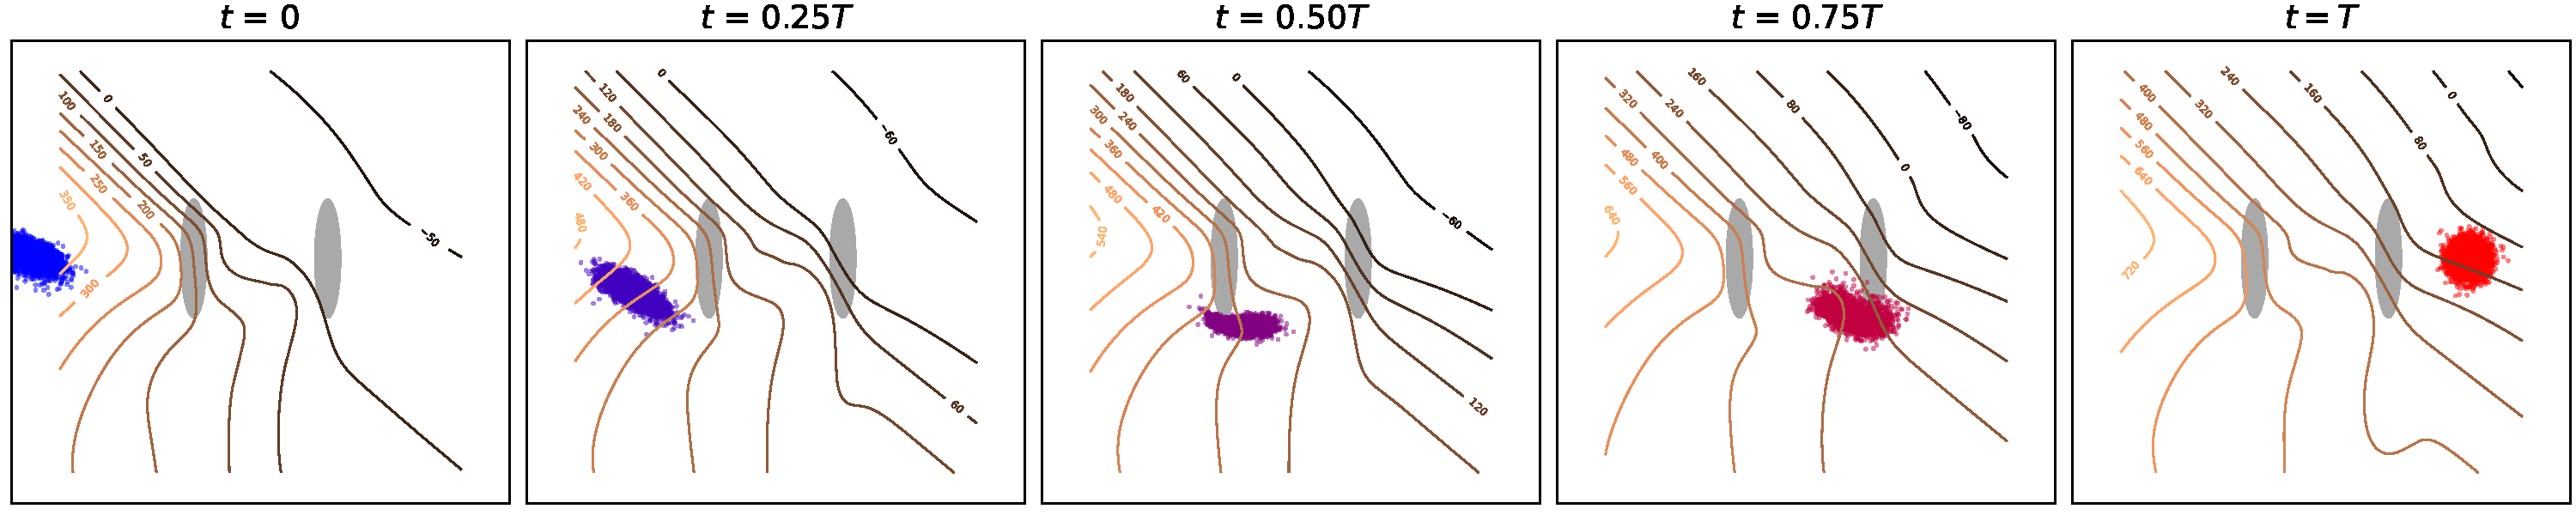
\includegraphics[width=0.8\textwidth]{Figures/stage10_double.pdf}
    \\
    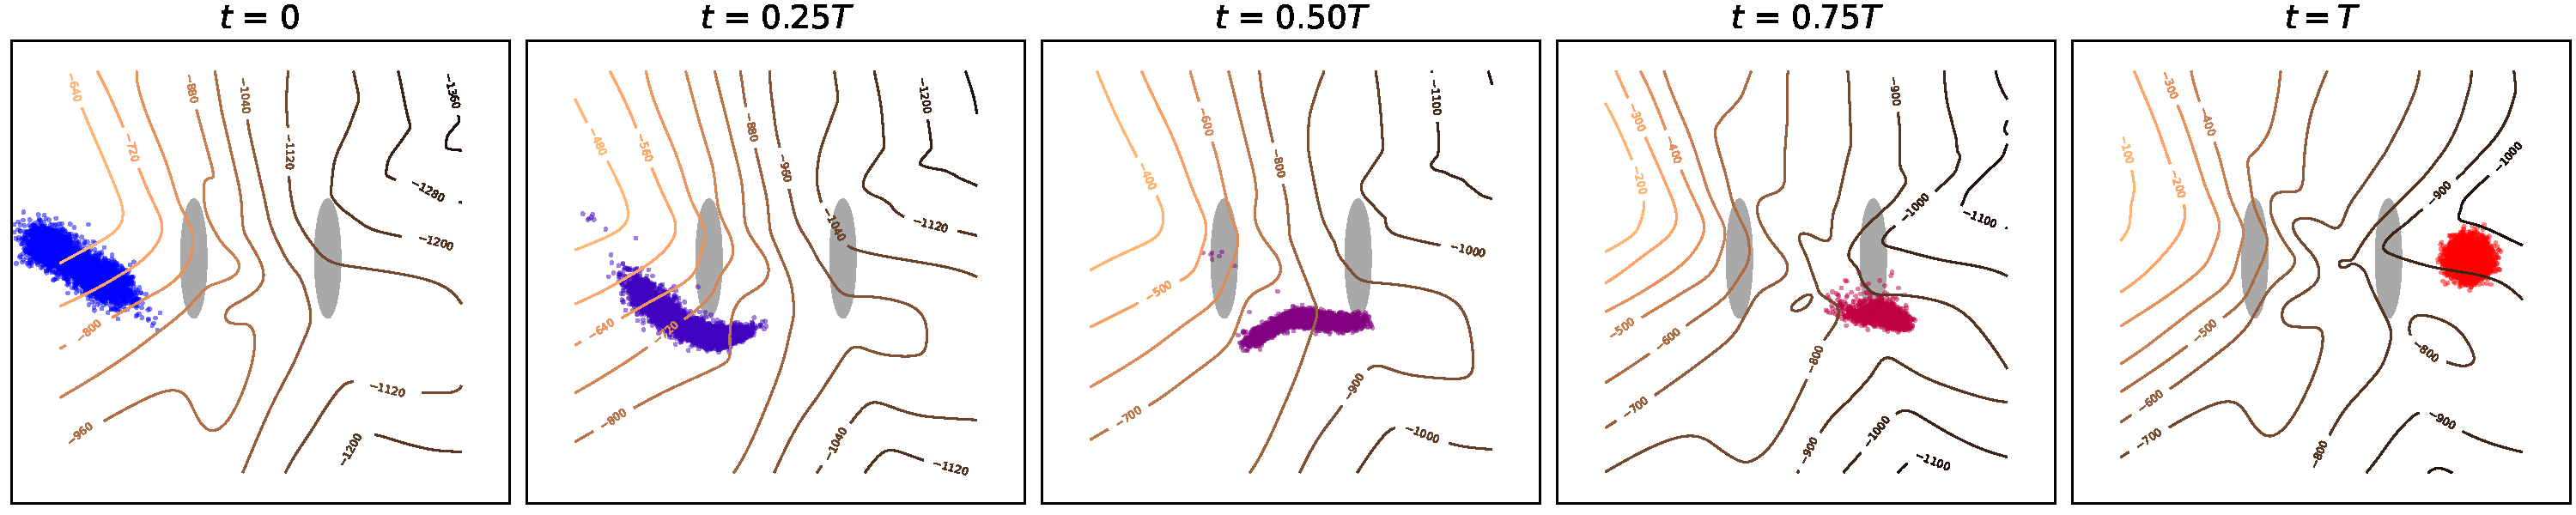
\includegraphics[width=0.8\textwidth]{Figures/stage20_double.pdf}
    \\
    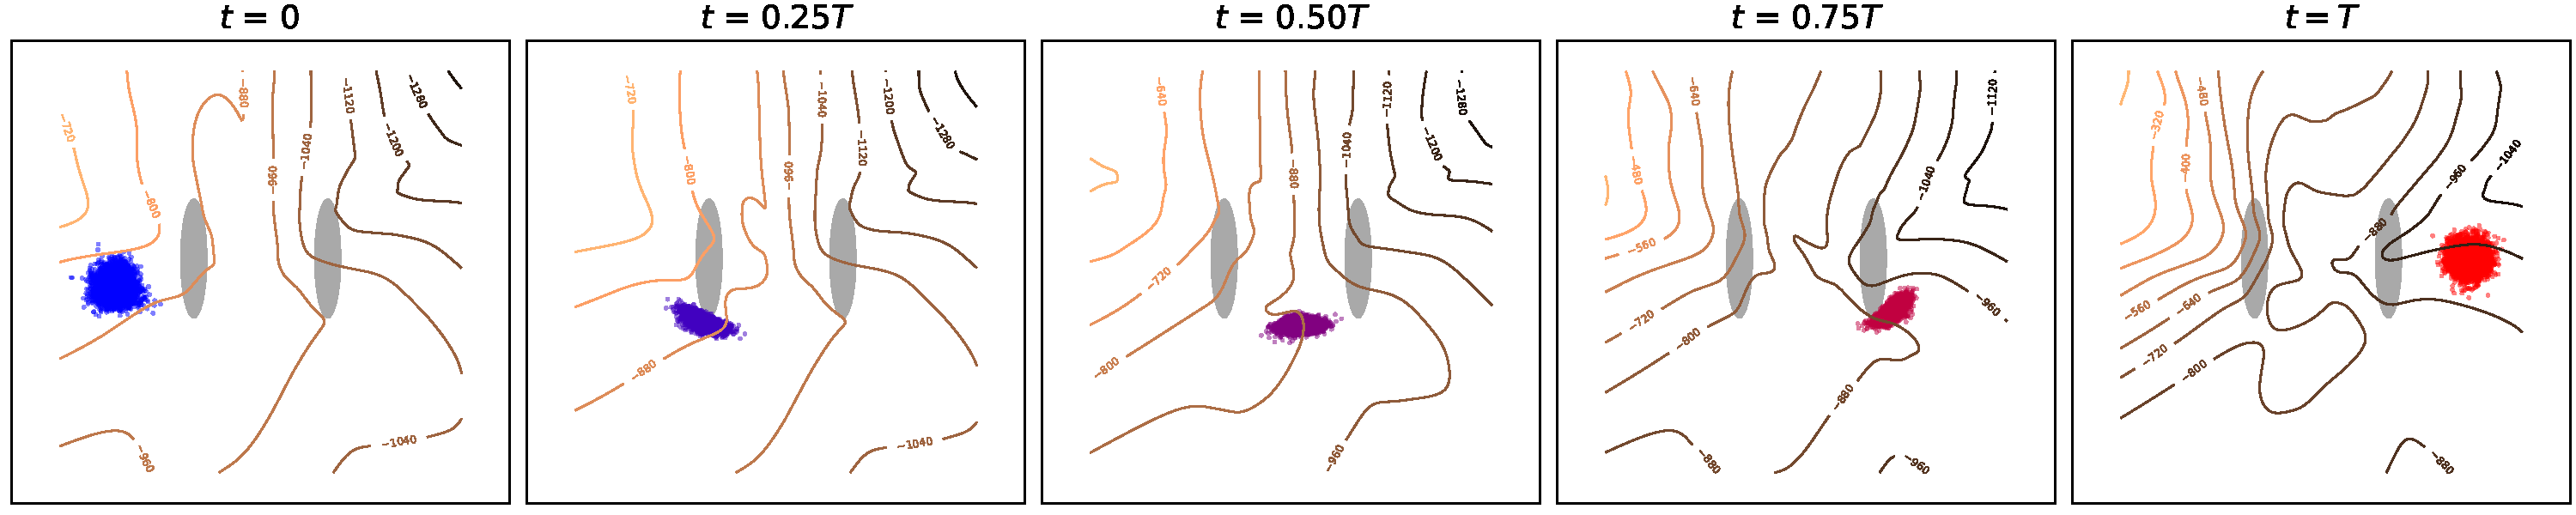
\includegraphics[width=0.8\textwidth]{Figures/stage40_double.pdf}
    \caption{Forward process. From top to bottom, Step n° $10, 20, 40$ of forward-backward pass.}
    \label{fig:fb_pass}
\end{figure}

On the Figure \ref{fig:fb_pass}, we can see that at step 10, half of the potential ("policy") has not been learned yet. At $t = 0.75T$, the distribution comes back up and is partially stuck against the second wall. At step 20, there is still some deformation of the distribution toward the interior of the obstacles, and the population is more spread out. Lastly, at step 40, the trajectory is optimized and compact.

Further work on our \href{https://github.com/gwatkinson/mva_sb_generative}{GitHub} highlight the impact of the congestion parameter K:
\[
F_{\rm congestion}(x, \rho) = \esp[y \sim \rho]{\frac{K}{\norme{x - y}^2 +1 }}
\]

It also underlines, as described in \cite{PhysRevLett.107.278001}, that adding an obstacle just before the exit help reduce the density.
\section*{Conclusion}

In conclusion, \cite{chen2023likelihood} have proposed a new method leveraging the power of Schrödinger Bridges in the context of generative modelling.
To do so, they had to use tools from Stochastic Optimal Control to solve complex PDEs.
In this process, they made a link between Schrödinger Bridges and Score-based Generative Models using the lower-bound of the log-likelihood developed in \cite{song2021maximum}.

We then explored the use of Schrödinger Bridges Forward Backward SDEs to solve the more general Mean-Field Games \cite{caluya2021wasserstein, liu2022deep}, that consist of the Hamilton-Jacobi-Bellman and Fokker-Planck PDEs, placing this method at the intersection of generative modelling, entropy regularized optimal transport and reinforcement learning.

The use of Schrödinger Bridges is an elegant solution to generative modelling, backed by a well-founded mathematical framework and detailed practical implementations.
However, it is hard to quantify if it actually outperforms current SGM models on generative tasks, without exhaustive and complex high dimensional experiments. But this approach is clearly interesting and allows for a broader interpretation of SGMs.

%%%%%%%%%%%%%%%%%%%%%%%%%%%%%%%%%%%%%%%%%%%%%%%%%%%%%%%%%%%

% Mail
% generative.modeling.mva@gmail.com



% Bibliographie
\clearpage
% \nocite{*}
\bibliographystyle{unsrtnat}
\addcontentsline{toc}{section}{Reference}
\bibliography{bibliography}



%%%%%%%%%%%%%%%%%%%%%%%%%%%%%%%%%%%%%%%%%%%%%%%%%%%%%%%%%%%%

\newpage
\appendix

\end{document}
